Bottom friction is a complex process because the bottom is generally a complex medium that can combine sand, mud, rocks, plants and animals. 
Also the bottom topography can strongly vary in the case of mobile sediments, with wave-generated ripples.  Finally,
flow in the bottom boundary layer may be turbulent, which requires a turbulence closure of 
the flow equations. 

The wave bottom boundary layer connects the region of potential flow where the oscillatory wave-induced velocity is given 
by eq. (\ref{vitesse}) to the sea bed where the velocity is zero. This boundary layer is very thin,  typically 10~cm or less. This is much less 
than the boundary layer of the mean current. As a result, when a current is present, the wave boundary layer also affects the 
friction for the current. 

We will consider here the case of a linear monochromatic waves. The velocity above the boundary layer is given by eq. (\ref{vitesse}), 
\begin{equation}
u_{+}(x,t)= \frac{\sigma a}{\sinh(kD)} \cos(k x -\omega t + \Theta_0),
\end{equation}
Because the wave propagates at the phase velocity $C$, the horizontal advection of any quantity $X$ by the 
velocity $u$ is $u \partial X /\partial x$, which can be neglected compared to  $\partial X /\partial t$ because the first term 
is $u/C$ smaller than the second, and $u/C$ is typically less than 0.2.
Let us define $ u_\delta(x,z,t)=\left\langle u(x,z,t)\right\rangle-u_{+}(x,t)$, in which the brackets $\langle . \rangle$ represent a Reynolds average, over the realizations of the turbulent flow. 

The conservation of the horizontal momentum component reads
\begin{equation}
\frac{\partial \widetilde{u}}{\partial t}=-\frac{1}{\rho_w}\frac{\partial
p}{\partial x} - \frac{\partial u_+}{\partial t} + G \label{BBL_qdm}
\end{equation}
with $G$ the divergence of the vertical momentum fluxes due to viscosity or turbulence, 
\begin{equation}
G=\nu \frac{\partial^2 \widetilde{u}}{\partial z^2} + \frac{\partial
\left<u'w'\right>}{\partial z}.\label{BBL_G}
\end{equation}

Because the thickness of the boundary layer  $\delta$  is much less than the wavelength, the pressure gradient in the boundary layer equals 
the pressure gradient outside the boundary layer, which is balanced by the acceleration,
\begin{equation}
-\frac{1}{\rho_w} \frac{\partial p}{\partial x}=\frac{\sigma^2 a}{\sinh(kD)} \sin(k x -\sigma
t)={\partial u_+}/{\partial t}.\label{BBL_pressure}
\end{equation}
This is another way to write the Bernoulli equation \citep[see also][]{Mei1989}.

Replacing (\ref{BBL_pressure}) in (\ref{BBL_qdm}) one obtains
\begin{equation}
\frac{\partial u_\delta}{\partial t}=  G,
\end{equation}
with the matching condition  
\begin{equation} 
u_\delta \rightarrow 
0 \quad \mathrm{for} \quad z \gg \delta.
\end{equation}


\section{Viscous solution}\label{wbbl_viscous}
The laminar situation is very interesting because it has an analytical solution 
that allows to show general properties of the boundary layer. 
In the laminar case $G=\nu {\partial^2 \widetilde{u}}/{\partial z^2}$  and the solution is
\begin{equation}
u_\delta (x,z,t)=\frac{\sigma a}{\sinh(kD)} \mathrm{e}^{-z_+} \cos\left(k x - \sigma t
-z_+\right)  \label{uvisc}
\end{equation}
with 
\begin{equation}
z_+=(z+h)/\sqrt{2 \nu/\sigma}=(z+h)/\delta,
\end{equation}
in which we have used the definition 
\begin{equation}
 \delta\equiv \sqrt{2 \nu/\sigma}
\end{equation}
that gives an order of magnitude of the boundary layer thickness. 


The full velocity profile is thus  $u=u^+ + u_\delta$.
Because of the $-z_+$  term in the phase, the velocity $u$ in the boundary layer has a phase ahead of the the free stream velocity $u^+$.
This phase advance grows with $z_+$ but it only impacts a smaller fraction of velocity for larger values of $z_+$.  This advance is due to the 
importance of the friction term in the momentum balance, which gets added to the pressure gradient and inertia. 
A linear friction for laminar flow is proportional to  $- u$  and thus in phase with the pressure gradient $\partial p / \partial x$,  whereas inertia $\rho_w \partial u/\partial t$ has a phase lags of 90$^\circ$.

From the velocity solution, we obtain the dissipation rate of wave energy per unit surface, 
as given by the work of the viscous stress. Once divided by the wave energy $E_t$ per unit surface, one gets the attenuation coefficient 
\begin{equation}
\beta_{\nu} = \frac{\left<\rho_w \nu u \partial u/\partial z\right>}{\rho_w g a^2/2}
\end{equation}
Using the solution in eq. (\ref{uvisc}) we get 
\begin{equation}
\frac{\partial u_\delta}{\partial z}=- \frac{\sigma a}{\sinh(kD)}  \frac{\mathrm{e}^{-z_+} }{\sqrt{2 \nu / \sigma}} \left[\cos\left(k x - \sigma t
-z_+\right) - \sin\left(k x - \sigma t
-z_+\right)\right] 
\end{equation}
in which only the first term correlates with  $u$, and gives 
\begin{equation}
\beta_{\nu} =-\frac{\sigma^3 \delta}{2 g \sinh^2(kD)}.
\end{equation}

The spectral dissipation rate is thus of the following form 
\begin{equation}
S_{\mathrm{bfric}}(\kb) =-\frac{\sigma^3 \delta}{2 g \sinh^2(kD)}  E(\kb) .
\end{equation}

As we have seen in chapter \ref{ch_momentum}, the dissipation of wave energy  also comes with a loss of momentum  at the rate 
$\beta_{\nu} E /C$ for a monochromatic wave train. So what happens to that momentum?


\section{Streaming}
Because momentum is conserved, we have to investigate where it goes, and thus look into the mean current. 
For this we also need the vertical velocity $w_\delta$ associated to $u_\delta$. It is simply given by the 
conservation of mass 
$\partial w_\delta /\partial z=-\partial u_\delta /\partial x$, with the result
\begin{equation}
w_\delta =-\frac{2 k \delta \sigma a }{\sinh(kD)} \mathrm{e}^{-z_+} \left[\cos\left(k x - \sigma t
-z_+\right) + \sin\left(k x - \sigma t
-z_+\right)\right].
\end{equation}

The phase shift between the boundary layer and the free stream has interesting consequences. Indeed, the conservation of
mean flow momentum is 
\begin{equation}
\frac{\partial \overline{u w}}{\partial z} =\nu \frac{\partial^2 U}{\partial z^2}.\label{stream_eq1}
\end{equation}

Following \cite{Phillips1977}, one easily gets  
\begin{equation}
\overline{\left(u+u_\delta \right) \left(w+w_\delta \right)} =
\frac{\sigma^2 a^2 k \delta}{4 \sinh^2(kD)}\left[\frac{2}{\delta} \mathrm{e}^{-z_+}  \sin(z_+) -1 
+ 2 \mathrm{e}^{-z_+} \cos z_+ - \mathrm{e}^{-2z_+}\right].\label{stream_eq2}
\end{equation}

As $z_+$ goes to very large values ($z+D \gg \delta$), the momentum flux goes to 
\begin{equation}
\lim_{z_+ \rightarrow \infty}  \rho_w \overline{u w}=- \frac{\rho_w \sigma^2 a^2 k \delta}{4 \sinh^2(kD)}.
\end{equation}
This is exactly the momentum lost by the waves per unit time and unit horizontal surface. Hence, the momentum lost by the waves is taken up by the mean flow, and the waves 
accelerate a near boundary `streaming current' that was first reported by \cite{Caligny1878}. The steady state corresponds to a situation in which the 
bottom friction for the mean current passes on this momentum to the sea floor \citep{Longuet-Higgins2005}. 

The integration of eq. (\ref{stream_eq1}) gives 
\begin{equation}
U(z)= \frac{\sigma a^2 k}{4 \sinh^2(kD)} \left[3 - 2 \left(z_+ + 2\right) \er^{- z_+} \cos z_+
- 2 \left(z_+ +2\right) \er^{- z_+} \sin z_+
                                            + \er^{-2 z_+} \right].\label{ruissellement_Eulerien}
\end{equation}

We can also update our estimation of the Stokes drift from chapter \ref{ch_momentum}, now using   $\widetilde{u}$ and
$\widetilde{w}$. This gives a mass transport velocity $\overline{U}^L=U+U_s$ \citep{Longuet-Higgins1953}, 
\begin{equation}
\overline{U}^L= \frac{\sigma a^2 k}{4 \sinh^2(kD)} \left[5 - 8  \er^{- z_+} \cos z_+ +3  \er^{-2 z_+} \right].
\end{equation}

We note that this mass transport velocity at the top of the boundary layer 
is \emph{independent} of the value of $\nu$, because the same viscosity appears in the 
wave dissipation and in the friction for the current. An infinitely small viscosity gives the 
same current at the top of the boundary layer as strong viscosity, only the thickness of the boundary layer changes, whereas there is no mean current for a zero viscosity.
The mass transport velocity reaches 2.5 times the Stokes drift we had estimated in chapter \ref{ch1b}. The 
effect of bottom friction on near-bed currents is thus considerable, which is very important for sediment transport. The velocity profiles are shown in figure \ref{fig_streaming}. 
%%%%%%%%%%%%% figure
\begin{figure}
\centerline{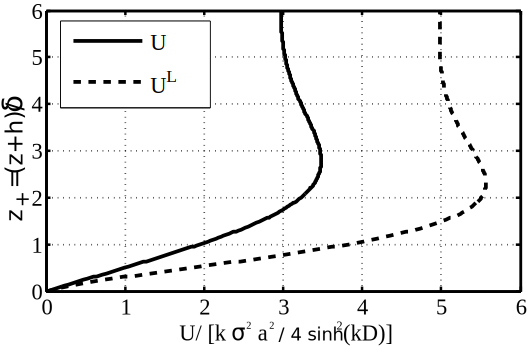
\includegraphics[width=0.7\textwidth]{FIGS_CH_BBL/streaming.pdf}}
  \caption{Mean current known as `streaming', induced by a monochromatic wave train.}{Profiles of the Eulerian mean and Lagrangian mean 
  velocities in the boundary layer for a constant viscosity $\nu$, with $\delta=\sqrt{2 \nu/\sigma}$.}
   \label{fig_streaming}
\end{figure}
%%%%%%%%%%%%% end of figure
The boundary layer introduces a significant change in the velocity profile between the bottom and  $z=-h+2.5 \delta$, where the velocity amplitude is maximum. 
The effective thickness of the boundary layer is thus close to  $2.5 \delta$. We note that the velocity profile is linear near the bed, 
and its vertical derivative gives the bottom stress,  
fond $\rho_w \nu \partial U/\partial z$, 
\begin{equation}
 \rho_w \nu \frac{\partial U}{\partial z} =\frac{\sigma^2 a^2 k \delta}{4 \sinh^2(kD)}=
\beta_{\nu} E /C.
\end{equation}

The loss of wave momentum to the bottom means that it is not the full radiation stress that is relevant for the change in sea level 
\citep{Longuet-Higgins2005,Ardhuin2006b}. 

In the presence of partially standing waves, the situation is a little more complicated, and the streaming is directed towards the surface elevation nodes, 
which is probably the cause of the formation of multiple sand bars  \citep{Heathershaw1982}.

\section{Turbulent boundary layer}
In practice the boundary layer is often turbulent, as very well observed in the laboratory by \cite{Jensen&al.1989}.
In the presence of a mean current, the wave boundary layer is thinner than the current boundary layer so that the waves define the roughness felt by the current. As a result
a change in wave height can lead to a change in tidal currents and tidal range  \citep{Wolf&Prandle1999}. 
As the effect of currents on the boundary layer is generally weaker, 
we will firs assume that the mean current is zero. 

Defining a Reynolds number from the free stream wave displacement amplitude $a_{\mathrm{orb}}$ and 
velocity amplitude $u_{\mathrm{orb}}$, 
\begin{equation}
 \mathrm{Re} = \frac{a_{\mathrm{orb}} u_{\mathrm{orb}}}{\nu}
\end{equation}
a transition to turbulence is observed for a smooth bottom for $\mathrm{Re} > 10^5$. For a wave period
of 10~s and monochromatic waves, this corresponds to a $a_{\mathrm{orb}} \simeq 0.5$~m. 
In practice the bottom roughness, even with fin sand, is enough to make the boundary layer turbulent 
for much lower amplitudes \citep{Jonsson1967}.
%%%%%%%%%%%%% figure
\begin{figure}
\centerline{\includegraphics[width=0.9\textwidth]{FIGS_CH_BBL/decollement.pdf}}
  \caption{Schematic of the flow in the boundary layer, showing the 
  importance of flow detachment from the boundary that induces a drag.}
  {Detachments can occur at all scales, from the grain size to ripples or coral elements \citep[e.g.][]{Monismith&al.2015}.}
   \label{fig_decollement}
\end{figure}
%%%%%%%%%%%%% end of figure
The bottom roughness is defined 
by all the elements of topography of horizontal scales less than the typical 
orbital amplitude $a_{b,{\mathrm{rms}}}$.

Following Prandtl, turbulence is characterized by eddies with a typical diameter $\kappa \delta$ at a distance 
$\delta$ from the bed.  These eddies turn around in time that is 
of the order of $\kappa \delta / u_\star$. The equivalent viscosity (or eddy viscosity)  $K_z$ is defined by a linear relation between 
the momentum flux and the velocity shear
\begin{equation}
u_\star^2=\overline{u^\prime w^\prime}= K_z
\partial u/ \partial z.
\end{equation}
When the  flux  $u_\star^2$ is constant, Prandtl's mixing length $l= \kappa (z+D)$ gives $K_z = \kappa (z+D) u_\star$, leading to
a log profile. Namely the solution of $\partial u/
\partial z = u_\star / (\kappa z)$ is 
\begin{equation}
u(z)=\frac{u_\star}{\kappa} \log\left(\frac{z}{z_0}\right).
\end{equation}

The eddies mix the flow on a time scale that is the $u_\star / l$. When this is is faster than the wave period we are in the boundary layer. 
Thus, an order of magnitude for the boundary layer thickness is given by 
\begin{equation}
              \delta=u_\star / (\kappa f) \approx
\sqrt{K_z/f}/\kappa.                                                            
\end{equation}

The friction velocity $u_\star$ is often related to the velocity $u_\infty$  outside of the boundary layer, with a friction coefficient
$f_w$, this gives  $u_\star^2=0.5 f_w u_\infty^2$. 
Experiments typically give a highly variable $f_w$, with values under 0.3. Typically  $f_w$ is a function of the ratio of the size of roughness elements 
$k_s$ and the orbital displacement $A$, and of the Reynolds number 
$Re$. In particular  $f_w$ decreases when  $A/k_s$ increases, and the wave boundary layer thickness is typically less than 10~cm.

Using eq. (\ref{BBL_qdm}) and (\ref{BBL_G}) a parameterization of the turbulent term $G$ following Prandtl mixing length ideas gives 
($u^\prime w^\prime = K_z
\partial u/
\partial z$) with $K_z = \kappa (z+D) u_\star$. This leads to the following equation \citep{Kajiura1968,Grant&Madsen1979},
\begin{equation}
\frac{\partial }{\partial z^\star} \left(z^\star \frac{\partial
u_\delta}{\partial z^\star}\right) + {\mathrm i} \widetilde{u} = 0,
\end{equation}
with $z^\star=\omega (z+D) / (\kappa u_\star)$.  This equation has an analytical solution. The boundary conditions of  $u_\delta$ going to zero when 
$z^\star$ is large gives 
\begin{equation}
u=\left[1-\frac{\ker (2\sqrt{z^\star}) + {\mathrm i} {\rm kei}
(2\sqrt{z^\star})}{\ker  (2\sqrt{z^\star_0})+  {\mathrm i} {\rm kei}
(2\sqrt{z^\star})} \right] u_+,
\end{equation}
where  $z^\star_0$ is the non-dimensional roughness  $z^\star_0=\omega
z_0 / (\kappa u_\star)$. For a smooth sandy bottom with well sorted grain sizes, 
\cite{Nikuradse1933} gives  $z_0=D_{50}/30$ where $D_{50}$ is the median sand grain size.

The Kelvin functions $\ker$ and ${\rm kei}$ are similar to a 
logarithm for $z^\star\rightarrow 0$, and oscillate for  $z^\star \rightarrow  \infty$. The general result is that the 
velocity amplitude is largest near the top of the boundary layer, and has a phase that leads the free stream oscillation  (figure \ref{fig_Wiberg_top}). 

Using this solution and taking the limit  $z^\star\rightarrow 0$, one gets the stress at the bottom and the wave energy dissipation rate, in the form of eq.  (\ref{roughness to friction 2}) below.
But we will first have to determine the bottom roughness.

This linear eddy viscosity model was extended to more realistic profiles, including a decrease of $K_z$ outside of the boundary layer and its variation with the wave phase. These modifications
have a very limited impact on the results \citep{Trowbridge&Madsen1984a,Jensen&al.1989,Wiberg1995,Davies&Villaret1999,Marin2004}. In particular the velocity profile is well reproduced by the 
linear and time-independent eddy viscosity (figure \ref{fig_Wiberg_top}). Still, there can be an impact on the shear stress at the bed, with consequences for the resuspension of sediments due, among other things, 
to the asymmetry between the acceleration and deceleration phases of the flow. Such flows are generally better captured by a $k-\omega$ turbulence closure \citep[e.g.][]{Marieu&al.2008}.
%%%%%%%%%%%%% figure
\begin{figure}
\centerline{\includegraphics[width=0.7\textwidth]{FIGS_CH_BBL/wiberg_1top.pdf}}
  \caption{Comparison of velocity profiles in the bottom boundary layer observed by \cite{Jensen&al.1989} at high Reynolds numbers and the model of \cite{Wiberg1995}.
  This case has a wave period of 10~s, with an amplitude of velocity oscillations of  1~m~s$^{-1}$. 
  The solid line represents model results using  $K_z=\kappa u_\star (z+D) {\mathrm e}^{-z^\star}$ that is time-independent, and the dashed line is the model 
  with a time-varying  $K_z$. Left panel: acceleration phase, right panel: deceleration. This figure is taken from \cite{Wiberg1995}. We note that the laboratory experiment of \cite{Jensen&al.1989} uses a
  U-shaped tube and thus does not include wave propagation effects such as the bottom streaming.} \label{fig_Wiberg_top}
\end{figure}
%%%%%%%%%%%%% end of figure


%Par ailleurs, la dissipation des vagues li\E9e au frottement sur le fond est
%donn\E9e par le travail de la tension de cisaillement sur le mouvement orbital
%$\overline{\tau u}$

%On retrouve aussi le ruissellement 
%Pour des profils de $K_z$ r\E9alistes et sur un fond rid\E9, il semble que la
%valeur maximale du courant de d\E9rive pr\E8s du fond soit effectivement de l'ordre
%de 2.5 fois $U_s (z=-H)$ \citep{Marin2004}. 

\section{Bottom roughness}
For a rocky seafloor, the bottom geometry may be complex, but at least it is fixed. In the case of sand, silt and mixtures the shape of the bottom 
and the associated roughness is modified by the flow and can also be strongly impacted by animals living in the sediment. Here we will discuss the case of 
a solid bottom, and leave the possibility of mud liquefaction for later \citep[e.g.][]{Jaramillo&al.2009}.

\subsection{Sand and ripples}
For a sandy seafloor, ripples are generally formed by the oscillatory wave motion, and these ripples determine the roughness and thus the dissipation rate 
of wave energy \citep{Zhukovets1963,Nielsen1992}. Starting from a flat seafloor, we can assume that  the roughness of the flow over sand grains is the same as measured by \cite{Nikuradse1933} 
in pipes in which sand was glued with lacquer. He found that $z_0=30 k_N$ where $k_N$ is the grain diameter. This scale $k_N$ is also called the Nikuradse roughness. In practice the 
sand grains may not have all the same diameter and it is customary to use the median grain size $D_{50}$. Another issue is that the bottom is not flat and thus it is not just the grains that contribute to the 
roughness (that part is called ``skin friction'') but there is also a ``form drag'' associated to the bottom geometry. This form drag generally varies with the amplitude of the flow characterized by the orbital diameter which is the 
length of orbits of water particles just outside the wave bottom boundary layer.

When the effects of a mean current are neglected, the bottom boundary layer can have three flow regimes, depending 
on the ratio of friction and buoyancy forces acting on sediment grains. This ratio is the Shields  number, and we generally 
consider the maximum value over a wave period defined as 
\begin{equation}
\psi _{{\rm max}}=\frac{f_{w}^{\prime }u_{{\rm max}}^{2}}{(s-1)gD},
\label{Shields}
\end{equation}
where $f_{w}^{\prime}$ is a skin friction factor, $s$ is the sediment grain density normalized by the density of seawater, e.g. $s=2.65$ for quartz, 
 $D$ is the grain size  \citep{Shields1936}.

When  $\psi _{{\rm max}}$ is low, the skin friction is not enough to set grains in motion and the bottom shape is fixed, possibly due to 
previous motions when waves were bigger. This is also called ``relict roughness''. This does not mean that the roughness $z_0$ is constant, 
because $z_0$ is a function of both the bottom shape and the flow. 
In that regime the dissipation of wave energy is weak. 

In a turbulent regime, the dissipation source term can be put in the following quasi-linear form, as proposed by \cite{Madsen&al.1990}, 
\begin{eqnarray}
\label{SandLforfriction}
%\startsubeqn
S_{\mathrm{fric}}\left(f,\theta\right) &=&\lambda \left(f\right)
\times E\left(f,\theta\right)
\label{model S} \\
\lambda \left(f\right) &=&-f_{e}u_{\rm b,rms}\frac{\left( 2\upi
f\right) ^{2}}{2g\sinh ^{2}\left( kD\right) },  \label{model lambda}
\end{eqnarray}
where the friction factor  $f_{e}$ is the ratio of the average dissipation rate and the cube of the root mean square velocity. 

As the orbital velocity increases, $\psi _{{\rm max}}$ may exceed the threshold $\psi _c$ and sand grains start moving. 
At that point, it only takes a few wave periods to form sand ripples. For quartz sand, the threshold $\psi _{c}$ ranges from 0.03 to 0.1, depending 
on the grain size $D$ \citep[e.g.][]{Soulsby1997}. The formation of these ripples enhances the form drag, and thus the dissipation 
rate of wave energy, corresponding to larger values of $f_{e}$. Random wave experiments by \cite{Madsen&al.1990} show that 
$f_{e}$ is maximum for  $\psi_{\rm rms} \simeq 1.2\psi _{c}$, where  $\psi_{\rm
rms}$ is estimated from the rms orbital velocity amplitude in  (\ref{Shields}) instead of $u_{{\rm max}}$.
For example, fine sand  ($D=0.15~$mm) in  25~m depth and a wave period $T_{p}$=12~s give this maximum dissipation for 
$H_{s}=1.5~$m. Beyond this threshold for sediment motion, any increase of the orbital velocity 
leads to smoother ripples and a reduction of $f_{e}$.

For very large values of  $\psi _{\rm max}$, of the order of  $10 \psi _{c}$
\citep{Li&Amos1999}, a layer of sediment called the `sheet flow' is fluidized and oscillates with the water column. At that stage, 
ripples are completely wiped out. Grain collisions become an important factor in the sediment layer. 
In that regime, the dissipation factor $f_{e}$ grows with 
$\psi$. The three regimes of relict roughness, actively formed ripples and sheet flow are illustrated in  figure \ref{fig three regimes}.
%%%%%%%%%%%%% figure
\begin{figure}
\centerline{\includegraphics[width=0.8\textwidth]{FIGS_CH_BBL/introduction_fig2.pdf}}
%\vspace{3.64in}
  \caption{Three regimes of the boundary layer over a sandy bottom}{(a) Relict roughness with possible contribution from benthic fauna.
  (b) ripple formation. (c)
sheet flow. The ocean wave wavelength $L$ and the depth are not to scale $L\approx 100$~m, compared to $\lambda \simeq 1$~m
for the ripple wavelength. Horizontal arrows represent the velocity profile under wave crests. Curvy arrows in  (b) 
represent the eddies in the wake of ripples.} \label{fig three regimes}
\end{figure}
%%%%%%%%%%%%% end of figure

Using dimensional analysis and numerical modeling, \cite{Andersen1999} showed that ripples 
self-organize to reach wavelengths of the order of 
$\lambda=0.63d$ where  $d$ is the orbital diameter of water parcels above the boundary layer, and their slopes are of the order of 15\%. 
This is typically observed for random waves in depths larger than 10~m, replacing  $d$ by 
$2^{1/2}d_{\mathrm{rms}}$ \citep{Traykovski&al.1999,Ardhuin&al.2002}. In very shallow water, it seems that ripple wavelengths are shorter and scale 
with the grain size \citep{Dingler1974,Wiberg&Harris1994}.

The determination of wave energy dissipation reduces to a parameterization of $f_{e}$ that must take into 
account ripples \citep{Graber&Madsen1988,Tolman1994,Ardhuin&al.2003a}.

%La plupart des mod\E8les de couche limite repr\E9sentent la
%turbulence par un profil vertical de viscosit\E9 turbulente (Kajiura,
%1968\nocite{Kajiura1968}; Grant et Madsen, 1979\nocite{Grant&Madsen1979};
%Weber, \nocite{Weber1991}1991\textit{a}, 1991\textit{b}\nocite{Weber1991b};
%voir \nocite {Wiberg1995} Wiberg, 1995, pour une discussion des diff\E9rents
%mod\E8les). Le fait que l'on puisse utiliser une seule valeur de la rugosit\E9
%$k_N$ pour l'ensemble du spectre a \E9t\E9 valid\E9 par Mathisen et Madsen
%(1999\nocite{Mathisen&Madsen1999}). En pratique, le terme de dissipation
%$S_{\mathrm{fric}}$ de l'\E9quation d'\E9volution du spectre est lin\E9aris\E9 par
%rapport au spectre d'\E9nergie (ou d'action) des vagues en supposant que le
%spectre des vagues est \E9troit et en utilisant un mod\E8le de couche limite pour
%les vagues monochromatiques `\E9quivalentes'.

It is common to use a representative grain size for the sediment, usually the median 
diameter 
$D_{50}$ for which we may estimate a critical Shields number $\psi _{c}$, above which grains start to move. It is also 
common to use root mean square values for the wave forcing at the top of the bottom boundary layer, in particular the 
orbital velocity $u_{\rm b,rms}$ and displacement $a_{\rm b,rms}$,
\begin{eqnarray}
\label{abandub}
%\stopsubeqn
%\startsubeqn
u_{\rm b,rms}^{2} &=&\int_{{\mathbf k}}\frac{8\upi ^{2}f^{2}}{\sinh ^{2}\left(
kD\right) }E\left( {\mathbf k}\right) d{\mathbf k},    \label{ub}
\\
a_{\rm b,rms}^{2} &=&\int_{{\mathbf k}}\frac{2}{\sinh ^{2}\left( kD\right) }%
E\left( {\mathbf k}\right) d{\mathbf k}.    \label{ab}
\end{eqnarray}
%%%%%%%%%%%%% figure
\begin{figure}[htb]
%\centerline{\psfig{file=aho2001_fig3.eps,width=0.85\textwidth}}
\centerline{\includegraphics[width=0.5\textwidth]{FIGS_CH_BBL/aho2001_fig3.pdf}}
%  \vspace{8.0cm}
  \caption{Example of dissipation factors $f_{e}$ as a function of the r.m.s. Shields
number $\psi_{\rm rms}$} {The solid line is the parameterization by \cite{Tolman1994}, for fine sand ($D_{50}=0.15~$mm), and a wave period
 $T=14~$s. This parameterization was adjusted to SHOWEX field data by  \cite{Ardhuin&al.2003b}. 
The dashed line correspond to an equivalent value of $f_{e}$ given by the JONSWAP parameterization, which does not 
take into account the varying bottom roughness.} \label{fig fe from psi}
\end{figure}
%%%%%%%%%%%%% end of figure

The boundary layer model gives a skin friction factor
$f_{w}^{\prime }$,  a Shields number  $\psi_{\rm rms} = f_{w}^{\prime
}u_{\rm b,rms}^{2}/\left[ g\left( s-1\right) D_{50}\right] $, and a total friction factor that includes skin 
and form drag  $f_{w}$, that is the ratio of the shear stress  $\tau$  and  $u_{\rm b,rms}^{2}$,
\begin{eqnarray}
%\stopsubeqn
%\startsubeqn
\frac{z_{0}}{l} &=&\sqrt{\frac{2}{f_{w}^{\prime }{\rm~ou~}f_{w}}}\frac{D_{50}
{\rm~ou~}k_{N}}{30\kappa ~a_{\rm b,rms}},  \label{roughness to friction 1}
\\
f_{w}^{\prime }{\rm~or~}f_{w} &=&\frac{\kappa ^{2}}{2\left[ \ker
^{2}\left( 2\sqrt{z_{0}/l}\right) +{\rm kei}^{2}\left( 2\sqrt{z_{0}/l}%
\right) \right] } \quad .    \label{roughness to friction 2}
\end{eqnarray}
where  $z_{0}/l$ is a non-dimensional roughness length,  $\kappa $ is von Karman's constant ($\kappa =0,4$), 
$\ker $ and  ${\rm kei}$ are the Kelvin functions of order  0 and 1.

When  $\psi_{\rm rms} /\psi _{c}<1,2$, $k_{N}$ is given by the relic roughness and may weakly increase with 
the orbital diameter  $a_{\rm b,rms}$ because larger horizontal scales contribute to the roughness when the flow 
amplitude increases. When  $\psi_{\rm rms} /\psi _{c}>1,2$ $k_N$
can be taken as the sum of a ripple roughness $k_r$ and a sheet flow roughness
`sheet flow' $k_s$. For example, 
 \cite{Madsen&al.1990} and \cite{Wilson1989} give
\label{krandks}
\begin{eqnarray}
k_{r} &=&a_{\rm b,rms}\times 1.5\left( \frac{\psi_{\rm rms}}{\psi _{c}}\right) ^{-2.5},
 \label{kr} \\
k_{s} &=&0.57\frac{u_{\rm b,rms}^{2.8}}{\left[ g\left( s-1\right) \right] ^{1.4}}%
\frac{a_{\rm b,rms}^{-0.4}}{\left( 2\upi \right) ^{2}}.    \label{ks}
\end{eqnarray}

Another approach to bottom friction that is completely empirical, goes back to the analysis of the JONSWAP experiment 
by \cite{JONSWAP}. In his analysis K. Hasselmann had initially thought that the bottom stress would be quadratic 
with a relation given by \cite{Hasselmann&Collins1968}, so that the dissipation rate may be cubic in the wave amplitude, with a theoretical formulation given for a Gaussian velocity distribution. The JONSWAP data 
contradicted this view, and  K. Hasselmann ended up fitting a dissipation rate that is proportional to the spectrum of 
the velocity variance at the bottom,
\begin{equation}
%\stopsubeqn
S_{\mathrm{fric,JONSWAP}}\left(f,\theta\right) =-\Gamma \left[ \frac{2\upi f}{%
g\sinh \left( kD\right) }\right] ^{2}E\left(f,\theta\right).  \label{JONSWAP}
\end{equation}
The only justification for this expression was that the near-bottom tidal current $\widehat{u}$ could have played a role
and would give $\Gamma = g c_b \widehat{u}$ where $c_b$ is the drag coefficient of \cite{Hasselmann&Collins1968}. The JONSWAP data gives a mean value $\Gamma =$ 0,038~m$^{2}$s$^{-3}$, but it ranges from 0.0019 to 0.160 ${\rm
m}^{2}{\rm s}^{-3}$). 
It may be surprising that this parameterization have been widely used, even in the absence of mean current. It is probably because, 
by chance, it follows the general trend over a sandy bottom shown in figure \ref{fig fe from psi}. However, it fails in many cases  (figure \ref{rides}).

As for the effect of a mean current, what is happening in the wave bottom boundary layer will be discussed in the next section. Other wave-turbulence interaction effects 
are probably similar to what is happening near the surface, with a production of turbulence kinetic energy due to the Stokes drift 
stretching of the turbulence, at the rate $\overline{u'w'}\partial U_s /\partial z$, which can be large in the presence of tidal currents.% (see chapter \ref{ch_vaguescourant3D}).

%%%%%%%%%%%%% figure
\begin{figure}[htb]
\centerline{\includegraphics[width=0.6\textwidth]{FIGS_CH_BBL/rides.pdf}}
  \caption{Sand ripples and wave dissipation}
  {Top: three ripple fields observed with a sidescan sonar, each square is 30 m across \citep{Ardhuin&al.2002}. Bottom: 
  comparison of modeled and measured wave heights, normalized by the measured wave height at the location of the Chesapeake Lighthouse in 18~m depth, during swell-dominated conditions for the SHOWEX experiment \citep{Ardhuin&al.2003b}. The left panel shows the case in which the model has no dissipation, and the modeled $H_s$ can be 4 times the measured value. The center panel uses the JONSWAP parameterization, with $\Gamma =$ 0,038~m$^{2}$s$^{-3}$, and the right panels are based on \cite{Grant&Madsen1979} as modified by 
  \cite{Tolman1994} and \cite{Ardhuin&al.2003a} to include ripple formation and relic ripple roughness. This last parameterization is now called the SHOWEX parameterization.}
  \label{rides}
\end{figure}
%%%%%%%%%%%%% end of figure

\subsection{Rocks}
The strong dissipation over coral reefs can be attributed, to a large extent, to the very large roughness of corals. \cite{Lowe&al.2007} 
and \cite{Monismith&al.2015} gave detailed analyses of this situation. 


\section{Joint wave and current boundary layers}
The joint interaction of waves, current and turbulence can be relatively complex and \cite{Madsen1994} has extensively studied this problem, showin that the roughness for random waves could be given by a single parameter. A recent review and analysis is given by \cite{Zou2004}.

The theory distinguishes a wave boundary layer $z+H <
\delta_{wc}$, in which the wave stress  $\tau_{w}=\rho_w  u_{\star w}^2$ and the current stress 
$\tau_{c}=\rho_w u_{\star c}^2$  add up to give a total stress $\tau_{wc}=\rho_w
u_{\star wc}^2$, that is the net momentum flux towards the bottom, and a thicker current-only boundary layer  $z+H > \delta_{wc}$ in which the stress is given by the current stress only  $\tau=\rho_w
\overline{u^\prime w^\prime}=\tau_{c}$.

Following the analysis by \cite{Grant&Madsen1979}, the Eulerian mean  horizontal momentum equation is 
\begin{equation}
\kappa \left|u_{\star c}\right| z \frac{\partial \widehat{u}}{\partial z} =
u_{\star c}^2  \quad \textrm{where} \quad \left(z+H\right) > \delta_wc,
\end{equation}
with the momentum mixed by eddies of sizes controled by the distance to the bottom, following  Prantl. 
Close to the bottom, turbulence comes from shear production by both the current and the wave-induced velocities so that 
the current velocity is mixed by this combined turbulence 
\begin{equation}
\kappa \left|u_{\star c}\right| z \frac{\partial \widehat{u}}{\partial z} =
u_{\star wc}^2  \quad \textrm{where} \quad \left(z+H\right) < \delta_wc.
\label{curr_wbbl}
\end{equation}


These two equations can be solved separately giving 
\begin{equation}
\widehat{u} =\frac{u_{\star c}}{\kappa} \ln \frac{z}{z_{0c}} 
\quad \textrm{where} \quad \left(z+H\right) > \delta_wc,
\end{equation}
and,
\begin{equation}
\widehat{u} =\frac{u_{\star c}}{\kappa} \frac{u_{\star c}}{u_{\star wc}} \ln
\frac{z}{z_{1c}}  \quad \textrm{where} \quad \left(z+H\right) <
\delta_wc.
\end{equation}

Because $\widehat{u}$ is continuous, we get 
\begin{equation}
\fbox{$\displaystyle z_{0c} = z_{0wc}^\epsilon \delta_{wc}^{1-\epsilon}.$}\label{z0c}
\end{equation}
where $z_{0wc}$ is the roughness for the wave motion, and $\epsilon=u_{\star c}/u_{\star
m}$ with $u_{\star m}$ the maximum combined friction velocity, defined by 
\begin{equation}
u_{\star m}^2 = u_{\star w m}^2 + u_{\star c}^2
\end{equation}
in which  $u_{\star w m}=\max(u_{\star w})$ for monochromatic waves. In the case of random waves, it is logical to use the  r.m.s. value. 

This theory thus gives a wave-induced modification of the bottom roughness applicable to the current. \cite{Mellor2002} showed that a wave-averaged numerical model could use an enhancement of the turbulent kinetic energy due to wave dissipation, and the resulting mean current profile is similar to the result of a $k-l$ turbulence closure with a modified bottom roughness. Such an approach can be extended to add other sources of turbulence like wave breaking, which may influence bottom friction in the surf zone 
 \citep{Feddersen&al.2003} .


The equation (\ref{curr_wbbl}) for  $z_{0c}$ misses the source of momentum due to wave dissipation, which is responsible for streaming. 
\cite{Mathisen&Madsen1996b} have thus modified the equivalent roughness to shift the velocity profile by  $-\widehat{u}(\delta_{wc})$, namely, 
\begin{equation}
z_{0a}=z_{0c} \exp \left[\kappa \widehat{u}(\delta_{wc})/u_{\star c})\right].
\end{equation}
Near the bottom this gives  $\widehat{u}(z)=u_{\star c}/\kappa \ln(z/z_0a) = u_{\star c}/\kappa  \ln(z/z_0c) -\widehat{u}(\delta_{wc})$.

% ln(a/b*exp(c))=ln(a)-ln(b)-c
This adjustment of the roughness gives a mean velocity  $\widehat{u}$ at the elevation $-H+\delta_{wc}$. 
In practice this may change the effective $z_0$ from  1 to 3~cm \citep{Mathisen&Madsen1996b}.
%  ... tr\E8s bien mais, comment calculer $\widehat{u}$ ? C'est tout
%l'enjeu de certains travaux r\E9cents (dont Davies et Villaret 1999, Marin 2004).


